
\item 
The asymptotic Bode magnitude plot of  minimum phase transfer function
G(s) is show below.\\

Consider the following two statements.\\ \\
 \textbf{Statement 1:} Transfer function G(s) has 3 poles and one zero \\
 \textbf{ Statement 2:} At very high frequency $(\omega \to \infty)$, the phase angle $ \angle G(j\omega)=-3\pi/2$ \\ \\
Which of the following is correct ? \\
(A) Statement 1 is true and Statement 2 is false.\\
(B) Statement 1 is false and Statement 2 is true.\\
(C) Both the statements are true.\\
(D) Both the statements are false.\\
\begin{figure}[htp]
	\centering
	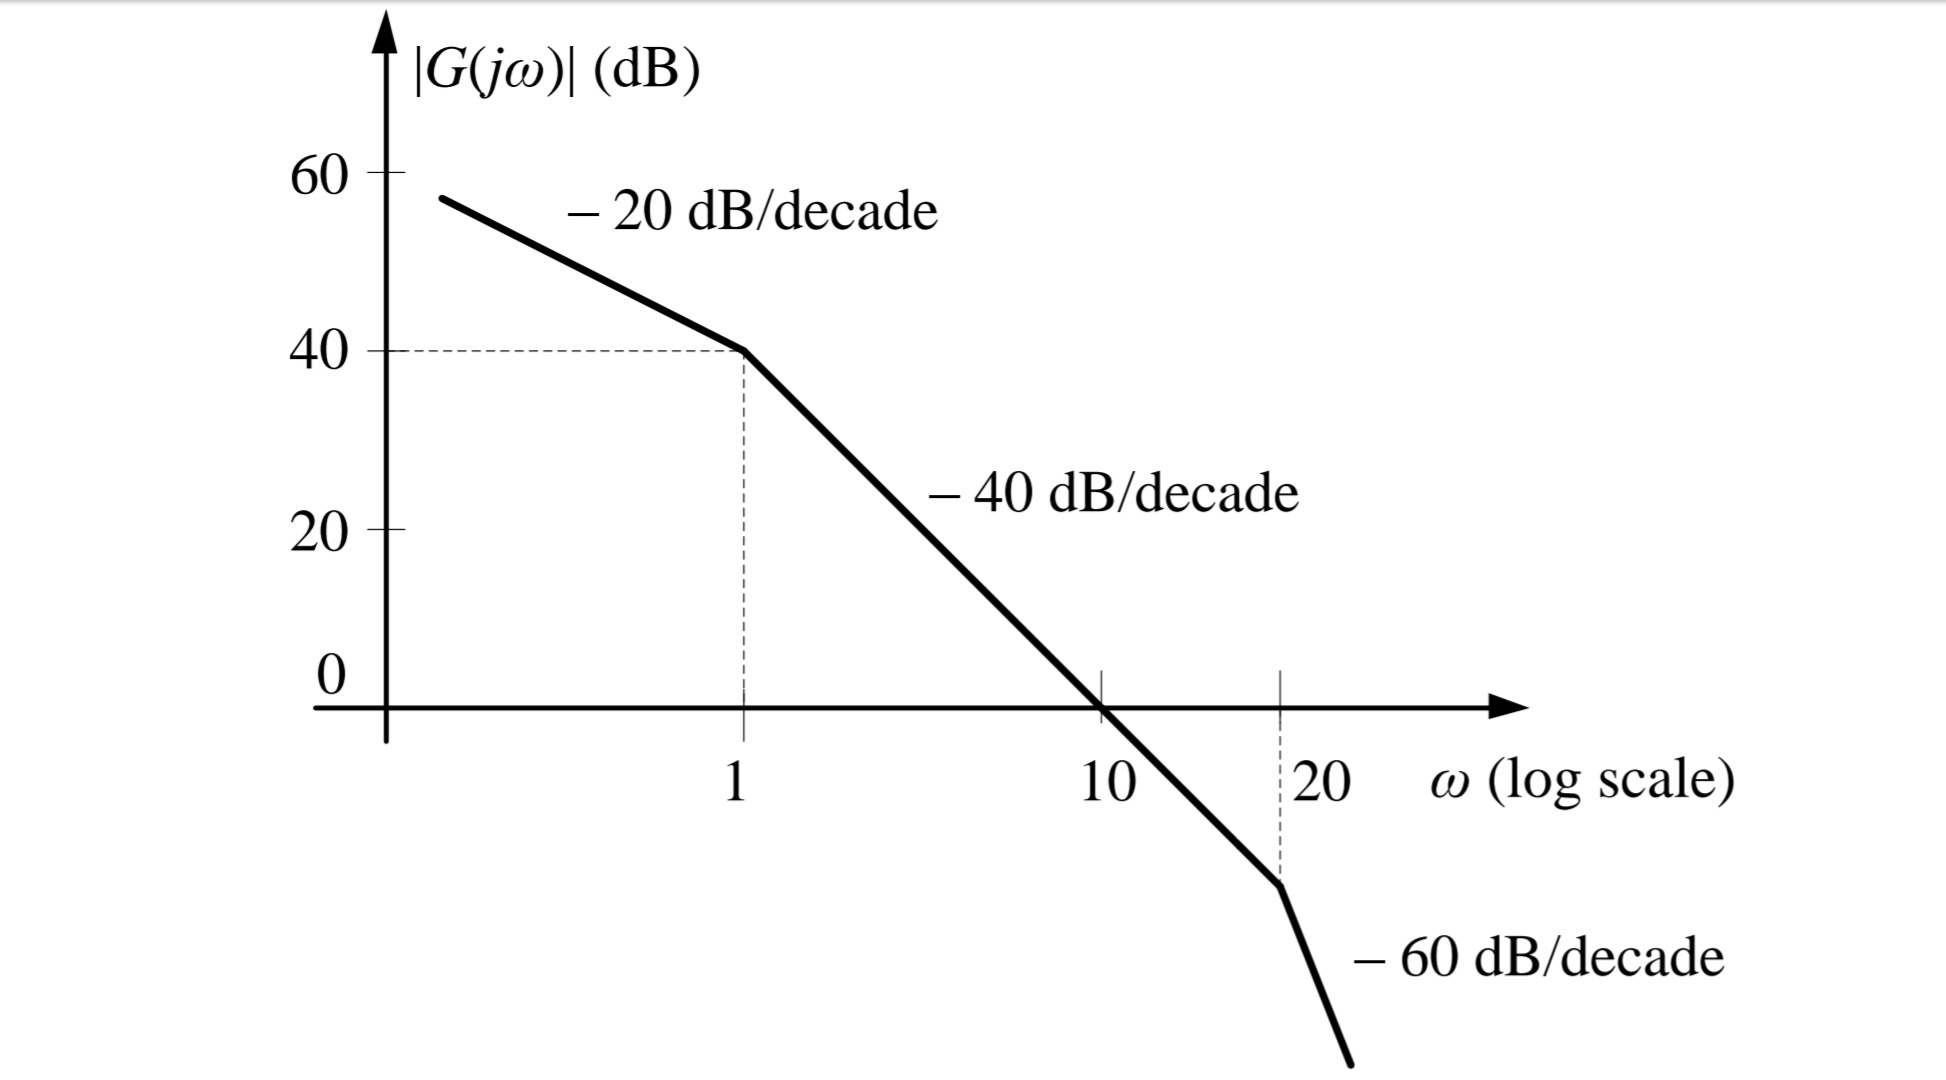
\includegraphics[width=1 \columnwidth]{./figs/pppp.eps}
	\caption{}
	\label{fig:galaxy}
\end{figure} 

\solution

Since, each pole corresponds to -20 dB/decade  
and each zero corresponds to +20 dB/decade.\\
Therefore, from the given Bode plot we can get the Transfer equation,
\begin{align}
G(s) = \frac{k}{s(1+s)(20+s)}
\end{align}

Now, from the Transfer equation we can conclude that,
there are three poles (0, -1 and -20 ) and no zeros.\\

$\therefore$ Statement 1 is false  ..........(1)

%------------------------------------------------

Calculating phase\\
Since we know that,\\
phase $ \phi $ is the sum of all the phases corresponding to each pole and zero.\\
phase corresponding to pole is =  
\begin{align}
-tan^{-1}( \frac{imaginary}{real})
\end{align} 
phase corresponding to zero is =
\begin{align}
 tan^{-1}( \frac{imaginary}{real})
 \end{align} 
%------------------------------------------------
Now take,
\begin{align}
 s = j\omega
  \end{align} 
  \begin{align}
 \Rightarrow  G(j\omega) =  \frac{k}{j\omega(1+j\omega)(20+j\omega)}
 \end{align} 
Therefore, 
\begin{align}
 \phi =  -tan^{-1}( {\frac{\omega}{0}}) - tan^{-1}(\omega) - tan^{-1}( \frac{\omega}{20})
 \end{align} 
 \begin{align}
  \phi =  - 90^\circ - tan^{-1}(\omega) - tan^{-1}( \frac{\omega}{20})
  \end{align} 
  \begin{align}
  \because \omega \to \infty
 \end{align} 
 \begin{align}
   \phi =   - 90^\circ - 90^\circ - 90^\circ
   \end{align} 
   \begin{align}
 \phi = -270^\circ
 \end{align} 
 \begin{align}
 \phi = -3\pi/2 
 \end{align} 
 $\therefore$ Statement 2 is true ........(2)\\
 thus, from (1) and (2) option (B) is correct.
 